\documentclass{../../../oss-apphys}

\usepackage[siunitx]{circuitikz} % to draw circuits!


\begin{document}
\genheader

\gentitle{C}{ELECTROSTATICS \& CAPACITORS}

\genmultidirections

%\gengravity

\raggedcolumns
\begin{multicols}{2}
  
  \begin{enumerate}[leftmargin=18pt]

  \item Two electric objects experience a repulsive force. What happens to that
    force if the distance between the objects is doubled?
    \begin{enumerate}[noitemsep,topsep=0pt,leftmargin=18pt,label=(\Alph*)]
    \item It decreases to one-fourth its value.
    \item It decreases to one-half its value.
    \item It stays the same.
    \item It doubles.
    \item It quadruples.
  \end{enumerate}

%  \item A pith ball is a tiny piece of Styrofoam that is covered with a
%    conductive paint. One pith ball initially has a charge of \SI{6.4e-8}{C},
%    and it touches an identical, neutral pith ball. After the pith balls are
%    separated, what is the charge on the pith ball that had the initial charge?
%    \begin{enumerate}[noitemsep,topsep=0pt,leftmargin=18pt,label=(\Alph*)]
%    \item\SI{6.4e-8}{C}
%    \item\SI{3.2e-8}{C}
%    \item\SI{0}{C}
%    \item\SI{-3.2e-8}{C}
%    \item\SI{-6.4e-8}{C}
%    \end{enumerate}
%
%  \item Glass becomes positively charged when it is rubbed with silk. Which
%    of the following is the best description of what’s happening?
%    \begin{enumerate}[noitemsep,topsep=0pt,leftmargin=18pt,label=(\Alph*)]
%    \item Electrons are rubbed off the glass onto the silk.
%    \item Electrons are rubbed off the silk onto the glass.
%    \item Protons are rubbed off the glass onto the silk.
%    \item Protons are rubbed off the silk onto the glass.
%    \item Neutrons in the glass have an affinity for positive charge.
%    \end{enumerate}
%    
%  \item Consider an isolated, neutral system consisting of wool fabric and a
%    rubber rod. If the rubber rod is rubbed with wool to become negatively
%    charged, what can be said about the wool fabric?
%    \begin{enumerate}[noitemsep,topsep=0pt,leftmargin=18pt,label=(\Alph*)]
%    \item It becomes equally negatively charged.
%    \item It becomes equally positively charged.
%    \item It becomes negatively charged but not equally.
%    \item It becomes positively charged but not equally.
%    \item In a neutral system, neither object can become charged.
%    \end{enumerate}

  \item An electron and a proton are separated by \SI{1.50e-10}{m}. If they are
    released, which one will accelerate at a greater rate, and what is the
    magnitude of that acceleration?
    \begin{enumerate}[noitemsep,topsep=0pt,leftmargin=18pt,label=(\Alph*)]
    \item The electron; \SI{1.12e22}{m/s^2}
    \item The proton; \SI{1.12e22}{m/s^2}
    \item The electron; \SI{6.13e18}{m/s^2}
    \item The proton; \SI{6.13e18}{m/s^2}
    \item They both accelerate at the same rate; \SI{1.02e-8}{m/s^2}
    \end{enumerate}

  \item Four charges are arranged at the corners of a square of side a as shown.
    Which of the following is true of the electric field and the electric
    potential at the center of the square?
    \begin{center}
      \begin{tikzpicture}[scale=2]
        \draw[dashed](0,0)--(1,0)--(1,1) node[midway,right]{$a$}
        --(0,1)--cycle;
        \draw[fill=black](.5,.5) circle(0.03);
        \draw[fill=white](0,0) circle(0.05) node[below left]{$-q$};
        \draw[fill=white](1,0) circle(0.05) node[below right]{$+q$};
        \draw[fill=white](0,1) circle(0.05) node[above left]{$+q$};
        \draw[fill=white](1,1) circle(0.05) node[above right]{$-q$};
      \end{tikzpicture}
    \end{center}
    \begin{tabular}{rll}
      & \underline{Electric Field} & \underline{Electric Potential}\\
      (A) & zero & zero \\
      (B) & $\frac{kQ}{a\sqrt{2}}$ & zero \\
      (C) & $\frac{kQ^2}{2a^2}$ &  $\frac{kQ}{2a}$\\
      (D) & zero &  $\frac{kQ}{\sqrt{2a}}$\\
      (E) & $\frac{kQ^2}{2a}$ & $\frac{kQ}{a\sqrt{2}}$
    \end{tabular}

    \columnbreak
    
  \item Which of the following diagrams best represents how you might rearrange
    the charges so that the electric field at the center would point directly
    toward the top of the page?
    \begin{enumerate}[noitemsep,topsep=0pt,leftmargin=18pt,label=(\Alph*)]
    \item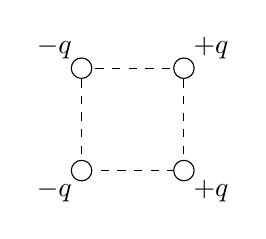
\begin{tikzpicture}[scale=1.3]
      \draw[dashed](0,0) rectangle(1,1);
      \draw[fill=white](0,0) circle(0.1) node[below left]{$-q$};
      \draw[fill=white](1,0) circle(0.1) node[below right]{$+q$};
      \draw[fill=white](0,1) circle(0.1) node[above left]{$-q$};
      \draw[fill=white](1,1) circle(0.1) node[above right]{$+q$};
    \end{tikzpicture}
    \item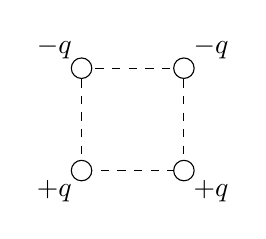
\begin{tikzpicture}[scale=1.3]
      \draw[dashed](0,0) rectangle(1,1);
      \draw[fill=white](0,0) circle(0.1) node[below left]{$+q$};
      \draw[fill=white](1,0) circle(0.1) node[below right]{$+q$};
      \draw[fill=white](0,1) circle(0.1) node[above left]{$-q$};
      \draw[fill=white](1,1) circle(0.1) node[above right]{$-q$};
    \end{tikzpicture}
    \item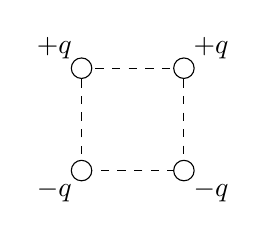
\begin{tikzpicture}[scale=1.3]
      \draw[dashed](0,0) rectangle(1,1);
      \draw[fill=white](0,0) circle(0.1) node[below left]{$-q$};
      \draw[fill=white](1,0) circle(0.1) node[below right]{$-q$};
      \draw[fill=white](0,1) circle(0.1) node[above left]{$+q$};
      \draw[fill=white](1,1) circle(0.1) node[above right]{$+q$};
    \end{tikzpicture}
    \item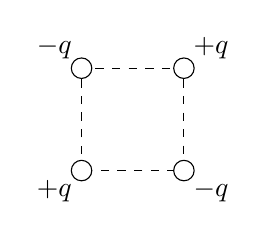
\begin{tikzpicture}[scale=1.3]
      \draw[dashed](0,0) rectangle(1,1);
      \draw[fill=white](0,0) circle(0.1) node[below left]{$+q$};
      \draw[fill=white](1,0) circle(0.1) node[below right]{$-q$};
      \draw[fill=white](0,1) circle(0.1) node[above left]{$-q$};
      \draw[fill=white](1,1) circle(0.1) node[above right]{$+q$};
    \end{tikzpicture}
    \item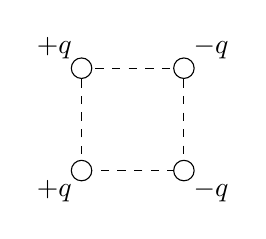
\begin{tikzpicture}[scale=1.3]
      \draw[dashed](0,0) rectangle(1,1);
      \draw[fill=white](0,0) circle(0.1) node[below left]{$+q$};
      \draw[fill=white](1,0) circle(0.1) node[below right]{$-q$};
      \draw[fill=white](0,1) circle(0.1) node[above left]{$+q$};
      \draw[fill=white](1,1) circle(0.1) node[above right]{$-q$};
    \end{tikzpicture}
    \end{enumerate}
    \columnbreak
    
  \item Three charges, $+Q$, $-Q$, and $+2Q$, are arranged in an equilateral
    triangle as shown. Which of the arrows below best represents the direction
    of the electric field at the center of the triangle?
    \begin{center}
      \vspace{-.1in}
      \begin{tikzpicture}[scale=2.5]
        \draw[dashed](0,0)--(1,0)--(.5,.866)--cycle;
        \draw[fill=black](.5,.289) circle(.03);
        \draw[fill=white](0,0) circle(.05) node[left]{$+Q\;$};
        \draw[fill=white](1,0) circle(.05) node[right]{$\;-Q$};
        \draw[fill=white](.5,.866) circle(.05) node[above]{$2Q$};
      \end{tikzpicture}
    \end{center}
    \begin{enumerate}[noitemsep,topsep=0pt,leftmargin=18pt,label=(\Alph*)]
    \item $\displaystyle\downarrow$
    \item $\displaystyle\uparrow$
    \item $\displaystyle\searrow$
    \item $\displaystyle\swarrow$
    \item $\displaystyle\nearrow$
    \end{enumerate}
  
  \item A non-conducting sphere does not have a uniform charge density, but the
    density $\rho$ varies with the distance $r$ from the center of the sphere
    according to the equation $\rho=\beta r$ where $\beta$ is a positive
    constant. The electric field inside the sphere ($r<R$) at a distance $r$
    from the center of the sphere is
    \begin{enumerate}[noitemsep,topsep=0pt,leftmargin=18pt,label=(\Alph*)]
    \item $\displaystyle\frac{\beta r^2}{12\epsilon_0}$
    \item $\displaystyle\frac{\beta r^3}{3\epsilon_0}$
    \item $\displaystyle\frac{\beta r}{2\epsilon_0}$
    \item $\displaystyle\frac{\beta r^2}{2\epsilon_0}$
    \item $\displaystyle\frac{\beta r^2}{4\epsilon_0}$
    \end{enumerate}
  
  \item The electric potential at the surface of the sphere from the last
    question is
    \begin{enumerate}[noitemsep,topsep=0pt,leftmargin=18pt,label=(\Alph*)]
    \item $\displaystyle\frac{\beta R^3}{12\epsilon_0}$
    \item $\displaystyle\frac{\beta R}{2\epsilon_0}$
    \item $\displaystyle\frac{\beta R^3}{3\epsilon_0}$
    \item $\displaystyle\frac{\beta R^2}{2\epsilon_0}$
    \item $\displaystyle\frac{\beta R^2}{4\epsilon_0}$
    \end{enumerate}

    \columnbreak
    
  \item According to Gauss's law, the net electric flux passing through a closed
    surface is
    \begin{enumerate}[noitemsep,topsep=0pt,leftmargin=18pt,label=(\Alph*)]
    \item positive if the flux is entering the surface
    \item negative if the flux is exiting the surface
    \item positive if the net charge inside the surface is zero
    \item negative if the net charge inside the surface is zero
    \item zero if the net charge inside the surface is zero
    \end{enumerate}

  \item According to Gauss's law, which of the following statements is true?
    \begin{enumerate}[noitemsep,topsep=0pt,leftmargin=18pt,label=(\Alph*)]
    \item It is possible to have a nonzero electric field, but zero electric
      flux.
    \item It is possible to have a nonzero electric flux, but zero electric
      field.
    \item It is possible to have a nonzero electric flux through a closed
      surface even if the enclosed charge in a surface is zero.
    \item If a surface is not closed (such as a sheet of paper), the flux
      through it must be zero.
    \item It is possible for charges located outside a closed surface to produce
      a net positive flux through the surface.
    \end{enumerate}

  \item Electric potential
    \begin{enumerate}[noitemsep,topsep=0pt,leftmargin=18pt,label=(\Alph*)]
    \item is a vector quantity that depends on the direction of the electric
      field
    \item is a scalar quantity that depends on the magnitude and sign of charges
      in the vicinity
    \item is a scalar quantity that depends on the square of the distance from
      the charges in the vicinity
    \item is a vector quantity that depends on the sign of the charges in the
      vicinity
    \item is a vector quantity that must point from high to low potential
    \end{enumerate}

  \item Gauss's law is most convenient to use when calculating an electric field
    due to
    \begin{enumerate}[noitemsep,topsep=0pt,leftmargin=18pt,label=(\Alph*)]
    \item charges outside a closed surface
    \item charges inside a closed surface that has high symmetry
    \item charges inside a closed surface that has low symmetry
    \item a potential difference that is negative
    \item a potential difference that is positive
    \end{enumerate}  
  \end{enumerate}

  \columnbreak
  
  \textbf{Question \ref{cube1}-\ref{cube2}}
  \begin{enumerate}[leftmargin=18pt,resume]
  \item A cube has sides of length $a$. The cube rests so that one side rests on
    the $x$-axis as shown. An electric field is established in the $x$-direction
    according to the function $E_x=bx^2$ , where $b$ is a positive constant.
    Which of the following statements is true?
    \label{cube1}
    \begin{center}
      \vspace{-.15in}
      \pic{.35}{cube.png}
    \end{center}
    \begin{enumerate}[noitemsep,topsep=0pt,leftmargin=18pt,label=(\Alph*)]
    \item\vspace{-.2in}There is a net charge inside the cube.
    \item There is no net charge inside the cube.
    \item The flux passing through the cube is negative.
    \item The flux passing through the cube is zero.
    \item The flux diminishes while passing through the cube.
    \end{enumerate}

  \item The charge inside the cube can be expressed by the equation
    \label{cube2}
    \begin{enumerate}[noitemsep,topsep=0pt,leftmargin=18pt,label=(\Alph*)]
    \item $\epsilon_0ba$
    \item $\epsilon_0ba^2$
    \item $\epsilon_0ba^3$
    \item $\epsilon_0ba^4$
    \item $\epsilon_0b^22a^2$
    \end{enumerate}

  \item Which of the following statements is true of electric field and
    equipotential lines?
    \begin{enumerate}[noitemsep,topsep=0pt,leftmargin=18pt,label=(\Alph*)]
    \item The electric field vector always points in the same direction as the
      equipotential lines.
    \item The electric field always points in the opposite direction of the
      equipotential lines.
    \item The electric field always points perpendicular to the equipotential
      lines.
    \item The electric field is always equal to the equipotential lines.
    \item Equipotential lines always form a circle around electric field lines.
    \end{enumerate}

    \columnbreak
    
  \item The potential $V$ as a function of distance $r$ for a particular charge
    distribution is given by the equation $V=ar^{-1}$. The electric field as
    a function of distance $r$ from the charge distribution is
    \begin{enumerate}[noitemsep,topsep=0pt,leftmargin=18pt,label=(\Alph*)]
    \item $1/3\;ar^{-3}$
    \item $2ar^{-1}$
    \item $ar^{-2}$
    \item $-a(\ln r)$
    \item $-ar^{-2}$
    \end{enumerate}
%  \vspace{-0.5in}
%  \begin{center}
%    \begin{tikzpicture}[scale=0.7]
%      \draw[fill=gray!60](0,0) circle(0.25);
%      \draw[dashed](0,0) circle(1);
%      \draw[dashed](0,0) circle(3);
%      \draw(0,0)--(1,0) node[pos=1,right]{$x$} node[midway,above]{$R$};
%      \draw[fill=black](1,0) circle(0.05);
%      \begin{scope}[rotate=230]
%        \draw(0,0)--(3,0) node[pos=1,right]{$y$} node[pos=0.7,right]{$3R$};
%        \draw[fill=black](3,0) circle(0.05);
%      \end{scope}
%    \end{tikzpicture}
    %  \end{center}
    
  \item A positively charged ring of radius $R$ is made of conducting material
    and has a charge $Q$ distributed uniformly around it. The center of the
    ring is located at point $0$ on the $x$-axis. The potential $V$ at a
    distance $3d$ from point $0$ on the $x$-axis is
    \begin{center}
      \vspace{-.1in}
      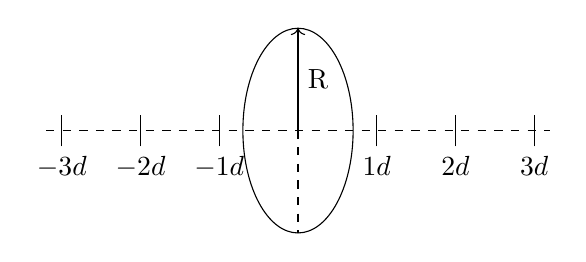
\begin{tikzpicture}
        \draw (0,0) ellipse (0.7 and 1.3);
        \draw[->](0,0)--(0,1.3) node[midway,right]{R};
        \draw[dashed](0,0)--(0,-1.3);
        \draw[dashed](-3.2,0)--(3.2,0);
        \foreach \x in {-3,-2,-1,1,2,3}{
          \draw(\x,-.2)--(\x,.2) node[pos=0,below] {$\x d$};
        }
      \end{tikzpicture}
    \end{center}

    \begin{enumerate}[noitemsep,topsep=0pt,leftmargin=18pt,label=(\Alph*)]  
    \item $\displaystyle V=\frac{kQ}{9d^2}$
    \item $\displaystyle V=\frac{kQ}{3d^2}$
    \item $\displaystyle V=\frac{kQ}{R^2+9d^2}$
    \item $\displaystyle V=\sqrt{\frac{kQ}{R^2+9d^2}}$
    \item $\displaystyle V=\frac{kQ}{\sqrt{R^2+9d^2}}$
    \end{enumerate}
  \end{enumerate}
\end{multicols}
\newpage

\genfreetitle{C}{ELECTROSTATICS \& CAPACITORS}{6}

\genfreedirections

% TAKEN FROM 2007 AP PHYSICS C EXAM FREE-RESPONSE QUESTION E&M 2
\begin{center}
  \pic{.3}{charges}
\end{center}
\begin{enumerate}[leftmargin=15pt]
\item In the figure above, a nonconducting solid sphere of radius a with charge
  $+Q$ uniformly distributed throughout its volume is concentric with a
  nonconducting spherical shell of inner radius $2a$ and outer radius $3a$ that
  has a charge $-Q$ uniformly distributed throughout its volume. Express all
  answers in terms of the given quantities and fundamental constants.
  \begin{enumerate}[leftmargin=15pt]
  \item Using Gauss's law, derive expressions for the magnitude of the
    electric field as a function of radius $r$ in the following regions.
    \begin{enumerate}[leftmargin=15pt]
    \item Within the solid sphere ($r<a$)
    \item Between the solid sphere and the spherical shell ($a<r<2a$)
    \item Within the spherical shell ($2a<r<3a$)
    \item Outside the spherical shell ($r>3a$)
    \end{enumerate}
  \item What is the electric potential at the outer surface of the spherical
    shell ($r=3a$)? Explain your reasoning.
  \item Derive an expression for the electric potential difference $V_X-V_Y$
    between points $X$ and $Y$ shown in the figure.
  \end{enumerate}
  \newpage

  % TAKEN FROM 2010 AP PHYSICS C EXAM FREE-RESPONSE QUESTION E&M 1
  \begin{center}
    \pic{.28}{circle}
  \end{center}
\item A charge $+Q$ is uniformly distributed over a quarter circle of radius
  $R$, as shown above. Points $A$, $B$, and $C$ are located as shown, with $A$
  and $C$ located symmetrically relative to the $x$-axis. Express all algebraic
  answers in terms of the given quantities and fundamental constants.
  \begin{enumerate}[leftmargin=15pt]
  \item Rank the magnitude of the electric potential at points $A$, $B$, and $C$
    from greatest to least, with number 1 being greatest. If two points have
    the same potential, give them the same ranking.

    \vspace{.1in}
    \underline{\hspace{.3in} } $V_A$ \hspace{.3in}
    \underline{\hspace{.3in} } $V_B$ \hspace{.3in}
    \underline{\hspace{.3in} } $V_C$
    
    \vspace{.1in}Justify your rankings.
  \end{enumerate}
  \vspace{.14in}
  Point $P$ is at the origin, as shown below, and is the center of curvature of
  the charge distribution.
  \begin{center}
    \pic{.28}{circle2}
  \end{center}
  \begin{enumerate}[leftmargin=15pt,resume]
  \item Determine an expression for the electric potential at point $P$ due to
    the charge $Q$.
    \vspace{\stretch{1}}
    
  \item A positive point charge $q$ with mass $m$ is placed at point $P$ and
    released from rest. Derive an expression for the speed of the point charge
    when it is very far from the origin.
    \vspace{\stretch{1}}
    \newpage
    
  \item On the dot representing point $P$ below, indicate the direction of the
    electric field at point P due to the charge $Q$.
    \begin{center}
      \begin{tikzpicture}[scale=1.2]
        \draw[dashed,->](-1,0)--(1,0) node[pos=1,right]{$x$};
        \draw[dashed,->](0,-1)--(0,1) node[pos=1,above]{$y$};
        \fill(0,0) circle(.1);
      \end{tikzpicture}
    \end{center}
  \item Derive an expression for the magnitude of the electric field at point
    $P$.
  \end{enumerate}
  \vspace{2in}
  
\item In the Bohr model of the hydrogen atom, the electron moves in a circular
  orbit of radius $r$ around the proton.
  \begin{enumerate}[leftmargin=15pt]
  \item Find an expression for the kinetic energy of the electron as a function
    of $r$. Show that at any distance $r$ the kinetic energy is half the
    potential energy.
  \item Evaluate kinetic energy $K$, potential energy $U$ and the total
    energy $W=K+U$ in electron volts for\\ $r=\SI{0.529e-10}{\metre}$, the
    radius of the electron's orbit in hydrogen. (The energy $|W|$ that must be
    supplied to the hydrogen atom to remove the electron is called the
    ionization energy.)
  \end{enumerate}
  \newpage

  % TAKEN FROM 2016 AP PHYSICS C EXAM FREE-RESPONSE QUESTION E&M 1
  \begin{center}
    \pic{.9}{potentials}
  \end{center}
\item Two point charges, $q_1$ and $q_2$, are fixed in place on the $x$-axis at
  positions $x_1=\SI{-1.00}{\metre}$ and $x_1=+\SI{0.50}{\metre}$,
  respectively. Charge $q_2$ has a value of $+2.0$ nC. Values of electric
  potential are illustrated by the given equipotentials in the diagram shown
  above, which is drawn to scale.
  \begin{enumerate}[leftmargin=15pt]
  \item Calculate the value of $q_1$.
  \item At point $C$ on the diagram, draw a vector representing the direction
    of the electric field at that point.
  \item Calculate the approximate magnitude of the electric field strength at
    point $D$ on the diagram.
  \item The equipotential labeled 0 V is the cross section of a nearly
    spherical surface. Calculate the electric flux for this surface.
    \newpage
    
  \item A proton is placed at point $A$ and then released from rest.
    \begin{enumerate}[leftmargin=15pt]
    \item Calculate the work done by the electric field on the proton as it
      moves from point $A$ to point $E$.
    \item Calculate the speed of the proton when it reaches point $E$.
    \end{enumerate}
  \item An electron is released from rest at point $B$. Which of the following
    indicates the direction of the initial acceleration, if any, of the
    electron?

    \vspace{.1in}
    \underline{\hspace{.3in}} Up\hspace{.3in}
    \underline{\hspace{.3in}} Down\hspace{.3in}
    \underline{\hspace{.3in}} Left\hspace{.3in}
    \underline{\hspace{.3in}} Right\hspace{.3in}
    \underline{\hspace{.3in}} Into the page\hspace{.3in}
    \underline{\hspace{.3in}} Out of the page

    \vspace{.1in}\underline{\hspace{.3in}} The direction is undefined since the
    acceleration is zero.

    \vspace{.1in}Justify your answer.
  \end{enumerate}
  \vspace{\stretch{1}}
  
%\item Two identical small spheres of mass $m$ are suspended from a common point
%  by threads of length $L$. When each sphere carries a charge $q$, each thread
%  makes an angle $\theta$ with the vertical as shown in the figure below.
%  \begin{enumerate}
%  \item Express charge $q$ in terms of $\theta$, $m$, $L$ and any other relevant
%    constants, and
%  \item Compute $q$ if $m=\SI{10}{\gram}$, $L=\SI{50}{\centi\metre}$ and
%    $\theta=\ang{10}$.
%  \end{enumerate}
%  \begin{tikzpicture}[scale=1.3]
%    \tikzstyle{balloon}=[ball color=red!60];
%    \fill[yellow!85!gray](-1.5,0) rectangle(1.5,0.15);
%    \draw[very thick,yellow](-1.5,0)--(1.5,0);
%    \draw[dashed,very thick,blue!80!gray](0,0)--(0,-4);
%    \draw[<->](0,-2.5) arc (270:285:2.5) node[midway,below]{$\theta$};
%    \draw[<->](0,-2.5) arc (270:255:2.5) node[midway,below]{$\theta$};
%    \begin{scope}[rotate=15]
%      \draw(0,0)--(0,-3.5) node[midway,right]{$L$};
%      \shade[balloon] (0,-3.5) circle (0.25) node[below]{$q$};
%    \end{scope}
%    \begin{scope}[rotate=-15]
%      \draw(0,0)--(0,-3.5) node[midway,left]{$L$};
%      \shade[balloon] (0,-3.5) circle (.25) node[below]{$q$};
%    \end{scope}
%  \end{tikzpicture}
%  \vspace{\stretch{1}}
   
%\item Five equal charges $Q$ are equally spaced on a semicircle or radius $R$
%  as shown in the figure below. Find the force on a charge $q$ located at the
%  center of the semi-circle. (Hint: Take advantage of symmetry.)
%  
%  \begin{tikzpicture}[scale=1.2]
%    \tikzstyle{balloon}=[ball color=yellow!40];
%    \draw(0,-1.75)--(0,3) node[pos=1,above]{$y$};
%    \draw(0,0)--(2.75,0) node[pos=1,right]{$x$};
%    \draw[->,rotate=120](0,0)--(1.75,0) node[midway,above right]{$R$};
%    \draw(0,1.75) arc (90:270:1.75);
%    \foreach \x in {0,45,...,180}
%    \shade[balloon,rotate=\x] (0,1.75) circle (0.2) node[left]{$Q\;\;$};
%    \shade[balloon] (0,0) circle(0.12) node[right]{$\;q$};
%  \end{tikzpicture}
%  \vspace{\stretch{1}}
%  \newpage
  
\item Two positive charges $+q$ are on the $y$ axis at $y=+a$ and $y=-a$.
  \begin{enumerate}[leftmargin=15pt]
  \item Show that the electric field on the $x$ axis is along the $x$ axis with
    $E_x=2kqx(x^2+a^2)^{-3/2}$.
  \item Show that near the origin, when $x\ll a$, $E_x\approx 2kqx/a^3$.
  \item Show that for $x\gg a$, $E_x\approx 2kq/x^2$.
  \item Explain why you should expect the result in (c) even before calculating
    it.
  \end{enumerate}
  A bead of mass $m$ with a negative charge $-q$ slides along a thread that
  runs along the $x$ axis.
  \begin{enumerate}[start=5,leftmargin=15pt]
  \item Show that for small displacements $x\ll a$, the bead experiences a
    restoring force that is proportional to $x$ and therefore undergoes
    simple harmonic motion.
  \item Find the period of the motion.
  \end{enumerate}
  \vspace{\stretch{4}}

%\item Using Gauss's law, find
%  \begin{enumerate}[leftmargin=15pt]
%  \item the electric field strength inside and outside of a uniformly charged
%    hollow sphere of radius $R$ and surface charge density $\sigma$ (charge
%    per unit area).
%
%  \item the electric field inside and outside an infinitely long cyclindrical
%    shell of charge of radius $R$ with charge discibution $\sigma$ (charge
%    per unit area).
%  \item the electric field strength inside and outside a infinitely long solid
%    cylinder of radius $R$ carrying a linear uniform charge density $\rho$
%    (charge per unit volume).
%  \end{enumerate}
%  %Hint: In all cases, think about where to put the Gaussian surface. Take
%  %advantage of symmetry.
%  \vspace{\stretch{1}}
%  \newpage
%
%\item For the circuit shown below, find
%  \begin{enumerate}[noitemsep]
%  \item The total equivalent capacitance between the terminals
%  \item The charge stored on each capacitor
%  \item the total stored charge
%  \end{enumerate}
%  \begin{tikzpicture}[scale=1.2,american voltages]
%    \draw[thick] (0,2) to[C=0.30<\micro\farad>,*-] (3,2)
%    to[C=1.0<\micro\farad>] (3,0) to[short,-*](0,0);
%    \draw[thick] (3,2)--(5,2) to[C=0.25<\micro\farad>,] (5,0)--(3,0);
%  \end{tikzpicture}
%  \vspace{\stretch{1}}
  \newpage
  
\item A parallel-plate capacitor has a capacitance $C_0$ and plate separation
  of $d$. To dielectric slabs of constants $\kappa_1$ and $\kappa_2$, each of
  thickness $d/2$ and having the same area as the plates, are inserted between
  the plates as shown in the figure below. When the free charge on the plates
  are $Q$,
  \begin{enumerate}[noitemsep]
  \item find the electric field in each of the dielectric
  \item find the potential difference between the plates
  \item show that the new capacitance is given by:
    $\displaystyle C=\frac{\kappa_1\kappa_2}{\kappa_1+\kappa_2}C_0$
  \end{enumerate}
  \pic{.2}{stacked.png}
  \vspace{\stretch{1}}

%\item Several point charges produce the equipotential lines shown.
%  \begin{enumerate}[noitemsep]
%  \item At which point on the diagram is the magnitude of the electric field
%    greatest? Explain.
%  \item Points C and D are approximately \SI{.02}{\metre} apart. Point F is
%    halfway between points C and D. What is the electric field at point F?
%  \item A \SI{5.}{\micro\coulomb} point charge is moved from point C to point
%    E, then to point D by an external force. Determine the work done by the
%    external force.
%  \end{enumerate}
%  \pic{.45}{equipotentials.png}
%  \vspace{\stretch{1}}

%\item A potential is given by
%  \begin{displaymath}
%    V(x,y,z)=\frac{kQ}{\sqrt{(x-a)^2+y^2+z^2}}
%  \end{displaymath}
%  \begin{enumerate}[noitemsep]
%  \item Find the components $E_x$, $E_y$ and $E_z$ of the electric field by
%    differentiating this potential function.
%  \item What simple charge distribution might be responsible for this potential?
%  \end{enumerate}
%  \vspace{\stretch{1}}
\end{enumerate}
\end{document}
